\documentclass[../main.tex]{subfiles}
\begin{document}

\chapter{Introduction}
\label{ch:introduction}


\section{Background}
\label{sec:background}

Multiple \glsxtrfull{ML} techniques rely on the manifold hypothesis \cite{fefferman_testing_2016}, which claims that high-dimensional data is sampled from a lower-dimensional manifold. One approach to leveraging this hypothesis is through the lens of computational topology, specifically \glsxtrfull{TDA}. TDA enables us to explore qualitative geometric properties of our datasets, such as identifying topological features (e.g., connected components, holes, and cavities) of the underlying manifold. Additionally, TDA can help us assess the relevance of observed features when additional complexity is introduced due to measurement or discretization issues.\\

Furthermore, as shown in \cite{hensel_survey_2021}, there is a growing interest in integrating TDA techniques into \glsxtrfull{DL} approaches, forming a new field referred to as \glsxtrfull{TopoML}. The survey showcases three distinct ways TDA tools are utilized in DL: incorporating topological feature extraction as a layer in a \glsxtrfull{NN} (either as an input or a hidden layer), imposing specific properties based on obtained topological information, and analyzing the topological properties of data and model architecture to assess specific characteristics of the trained model.\\


In our case, we will primarily focus on the second option—imposing certain properties through what we term "topological regularization." Specifically, we will expand upon the work proposed by Hofer \etal \cite{hofer_densified_2021}, where they demonstrate that imposing topological densification of each class distribution can enhance generalization capabilities. The main concept is to condense the density function of each class in the latent space, improving the likelihood of having each class distribution contained within its decision region. The authors of the paper observed that this property could be enforced by using an algebraic topology construction called Persistent Homology.\\

One of the main fields that have studied the properties of latent spaces of ML models is Representation Learning. Furthermore, one of the main topics of interest in this field is to analyze the similarities of latent representation between networks. It has been shown in \cite{moschella_relative_2022} that by using ``relative latent representations,'' we can increase the similarities between latent spaces. The relative latent representation is obtained as follows: let $S\subset\mathcal{X}$ a dataset, $\varphi: \mathcal{X} \to \mathcal{Z}$ the feature extractor component of your network, and $\mathcal{A}=\{a_1, ..., a_k\}\subset\mathcal{X}$ a set of points called \emph{anchors}. Then for any similarity function $sim$ we define the relative representation of a point $x\in S$  w.r.t. $\mathcal{A}$ as
\[
(sim(\varphi(x), \varphi(a_1)), ..., sim(\varphi(x), \varphi(a_k))\in \mathbb{R}^k.
\]

Furthermore, the authors demonstrated that this technique enables zero-shot stitching, meaning that models with different architectures, datasets, or seeds can be combined without additional fine-tuning, as illustrated in Figure~\ref{fig:crossDomainScheme_intro}.\\

\begin{figure}[ht!]
     \centering
    \begin{subfigure}[b]{0.45\textwidth}
         \centering
         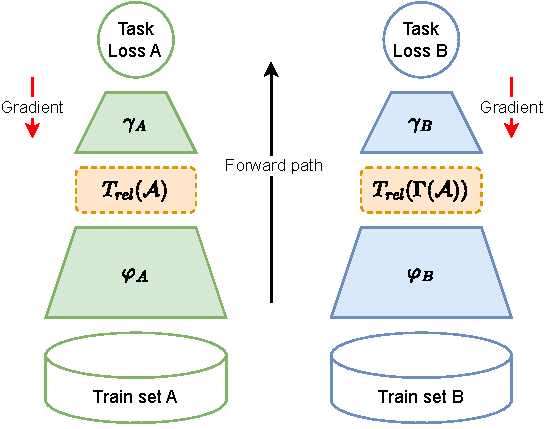
\includegraphics[width=\textwidth]{figures/bg/relativeTrainScheme.pdf}
        \caption{Train w/ relative transformations.}
         \label{fig:relTrainScheme_intro}
     \end{subfigure}\hfill
      \begin{subfigure}[b]{0.45\textwidth}
         \centering
         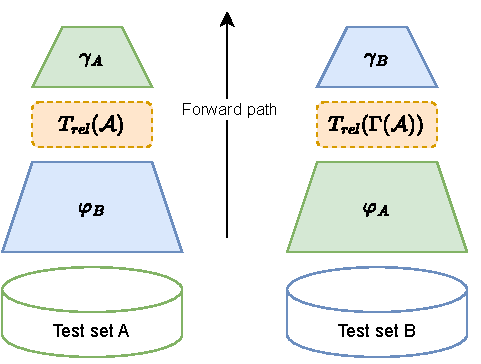
\includegraphics[width=0.9\textwidth]{figures/bg/relativeStitchScheme.pdf}
        \caption{Model stitching}
         \label{fig:relStitchScheme_intro}
     \end{subfigure}
    \caption{Cross-domain model stitching training and testing}
    \label{fig:crossDomainScheme_intro}
\end{figure}

For further mathematical background and detailed explanations of the described methods, please refer to Chapter~\ref{ch:background}.

\section{Problem}
\label{sec:problem}


The main objective of this project is to try to expand the work proposed on \cite{hofer_densified_2021} into the setup proposed on \cite{moschella_relative_2022}, so we can have a better understanding of how these intrinsic representation regularization techniques interact with novel latent space representations.

% Research Question
\subsection{Research question}
\label{sec:researchQuestion}

Therefore our main research question is: \emph{To what extent does the application of the topological regularization method described in \cite{hofer_densified_2021} impact the classification performance of zero-shot stitching when utilizing relative latent representations \cite{moschella_relative_2022}?}

\section{Purpose}

One of the purposes of this project is to showcase a brief introduction to TDA so that anyone with a ML background can comprehend the main philosophy and methodology proposed in this novel field of Topological Machine Learning. Additionally, this work will be valuable for researchers interested in transfer learning and representation learning as it explores the significance of latent space topology in the context of zero-shot stitching.


\section{Goals}

Considering that the chosen topological regularization technique \cite{hofer_densified_2021} requires a supervised classification setup, our focus will be on studying the zero-shot stitching of encoders and decoders that are both fine-tuned with a relative representation. This differs from the approach presented in \cite{moschella_relative_2022}, where only the decoder is fine-tuned using the relative representation while the encoder remains frozen. Consequently, our main goals are as follows:

\begin{itemize}
    \item Analyze the performance of zero-shot stitching after fine-tuning both the encoder and decoder with relative representation.
    
    \item Evaluate the performance when training with topological regularization and the relative representation. This entails the following tasks:

    \begin{itemize}        
        \item Assess the accuracy of zero-shot stitching in this setup.

        \item Assess whether we obtain better accuracy of the zero-shot stitching if we apply the topological regularization before or after the relative representation transformation.

        \item Assess the relevance of the used metric for the topological regularization.
    \end{itemize}
\end{itemize}

Lastly, the construction of the relative representation is primarily based on empirical evidence suggesting that, in certain cases, we can achieve latent representations that are nearly isometric \cite{moschella_relative_2022}. Therefore, an additional objective of this project is to provide a theoretical explanation for this claim and obtain new empirical results to support it. By accomplishing this, we can establish the theoretical validity of the relative transformation and gain valuable insights into the latent space of our network.


\section{Research Methodology}
We will now provide a concise overview of the methodology employed to achieve the objectives outlined in this project. A more in-depth explanation of the methods can be found in Chapter~\ref{ch:methods}.\\

Firstly,  we will enhance the theoretical foundation of the relative representation by leveraging specific characteristics of activation functions. Additionally, we will conduct novel empirical analyses to examine the similarities within the latent space across different initializations. This will involve both numerical and visual approaches. For numerical analysis, we will utilize standard metrics such as CKA while also introducing new metrics based on the Frobenius norm of the distance matrix. For visual analysis, Procrustes analysis will be employed to visually illustrate the optimal alignment of two latent spaces. These experiments will be conducted on an autoencoder and a CNN trained on the CIFAR10 dataset.\\

Upon validating the construction of the relative representation through these initial experiments, we will proceed to replicate selected experiments from \cite{moschella_relative_2022}, adapting them to our new setups. Specifically, we will replicate the Amazon review classification experiment using cross-lingual stitching. Throughout these experiments, we will compare different techniques for combining the relative transformation with Hofer's topological regularization. Furthermore, we will explore the potential advantages of using alternative metrics for constructing the Vietoris-Rips filtrations.

\section{Delimitations}
Our primary objective is to evaluate the impact of combining the previously defined methods through ablation studies rather than analyzing their performance under ideal conditions. Considering this objective and taking into account our time and computational limitations, we will not extensively tune hyperparameters as long as we can draw meaningful conclusions.


Furthermore, due to our computational constraints, we acknowledge that studying zero-shot stitching across different architectures and seeds is beyond the scope of this project. Additionally, to accommodate our computational limitations and maximize the number of tasks we can complete, we will utilize a 1\% sub-sample of the original training dataset instead of the 25\% sub-sampling approach employed in the original paper \cite{moschella_relative_2022}.


\section{Structure of the thesis}

The structure of this Thesis is organized as follows:
\begin{itemize}
    \item Chapter~\ref{ch:background} provides the essential background information, covering mathematical concepts such as simplicial complexes, homology, and persistence. It also explores related work in the field of Topological Machine Learning, representation similarity, and model stitching.

    \item Chapter~\ref{ch:methods} presents the research methodology, starting with a clear problem formulation. It then describes the conducted experiments and provides methodological justifications for their design.

    \item Chapter~\ref{ch:resultsAndAnalysis} presents the results obtained from the experiments and provides a thorough analysis of these findings.

    \item Chapter~\ref{ch:discussion} engages in further analysis, offering additional insights, opinions, and hypotheses concerning the methodology and the results obtained in this project.

    \item Chapter~\ref{ch:conclusionsAndFutureWork} concludes the thesis by summarizing the key conclusions derived from the research. It acknowledges the limitations of the study and proposes future avenues for further investigation. This chapter also includes reflections regarding the  environmental and socioeconomic implications of this work.
\end{itemize}

\end{document}